\documentclass{article}

\usepackage{graphicx}
\usepackage{tikz}
\usepackage{tikzsymbols}
\usetikzlibrary{calc,patterns,shapes.geometric}
\pagestyle{empty}
\usepackage[margin=0pt]{geometry}
\geometry{papersize={14in,12in}}

\def\centerarc[#1](#2)(#3:#4:#5){\draw[#1] ($(#2)+({#5*cos(#3)},{#5*sin(#3)})$) arc (#3:#4:#5);}

\begin{document}
	\begin{figure}
		\centering
		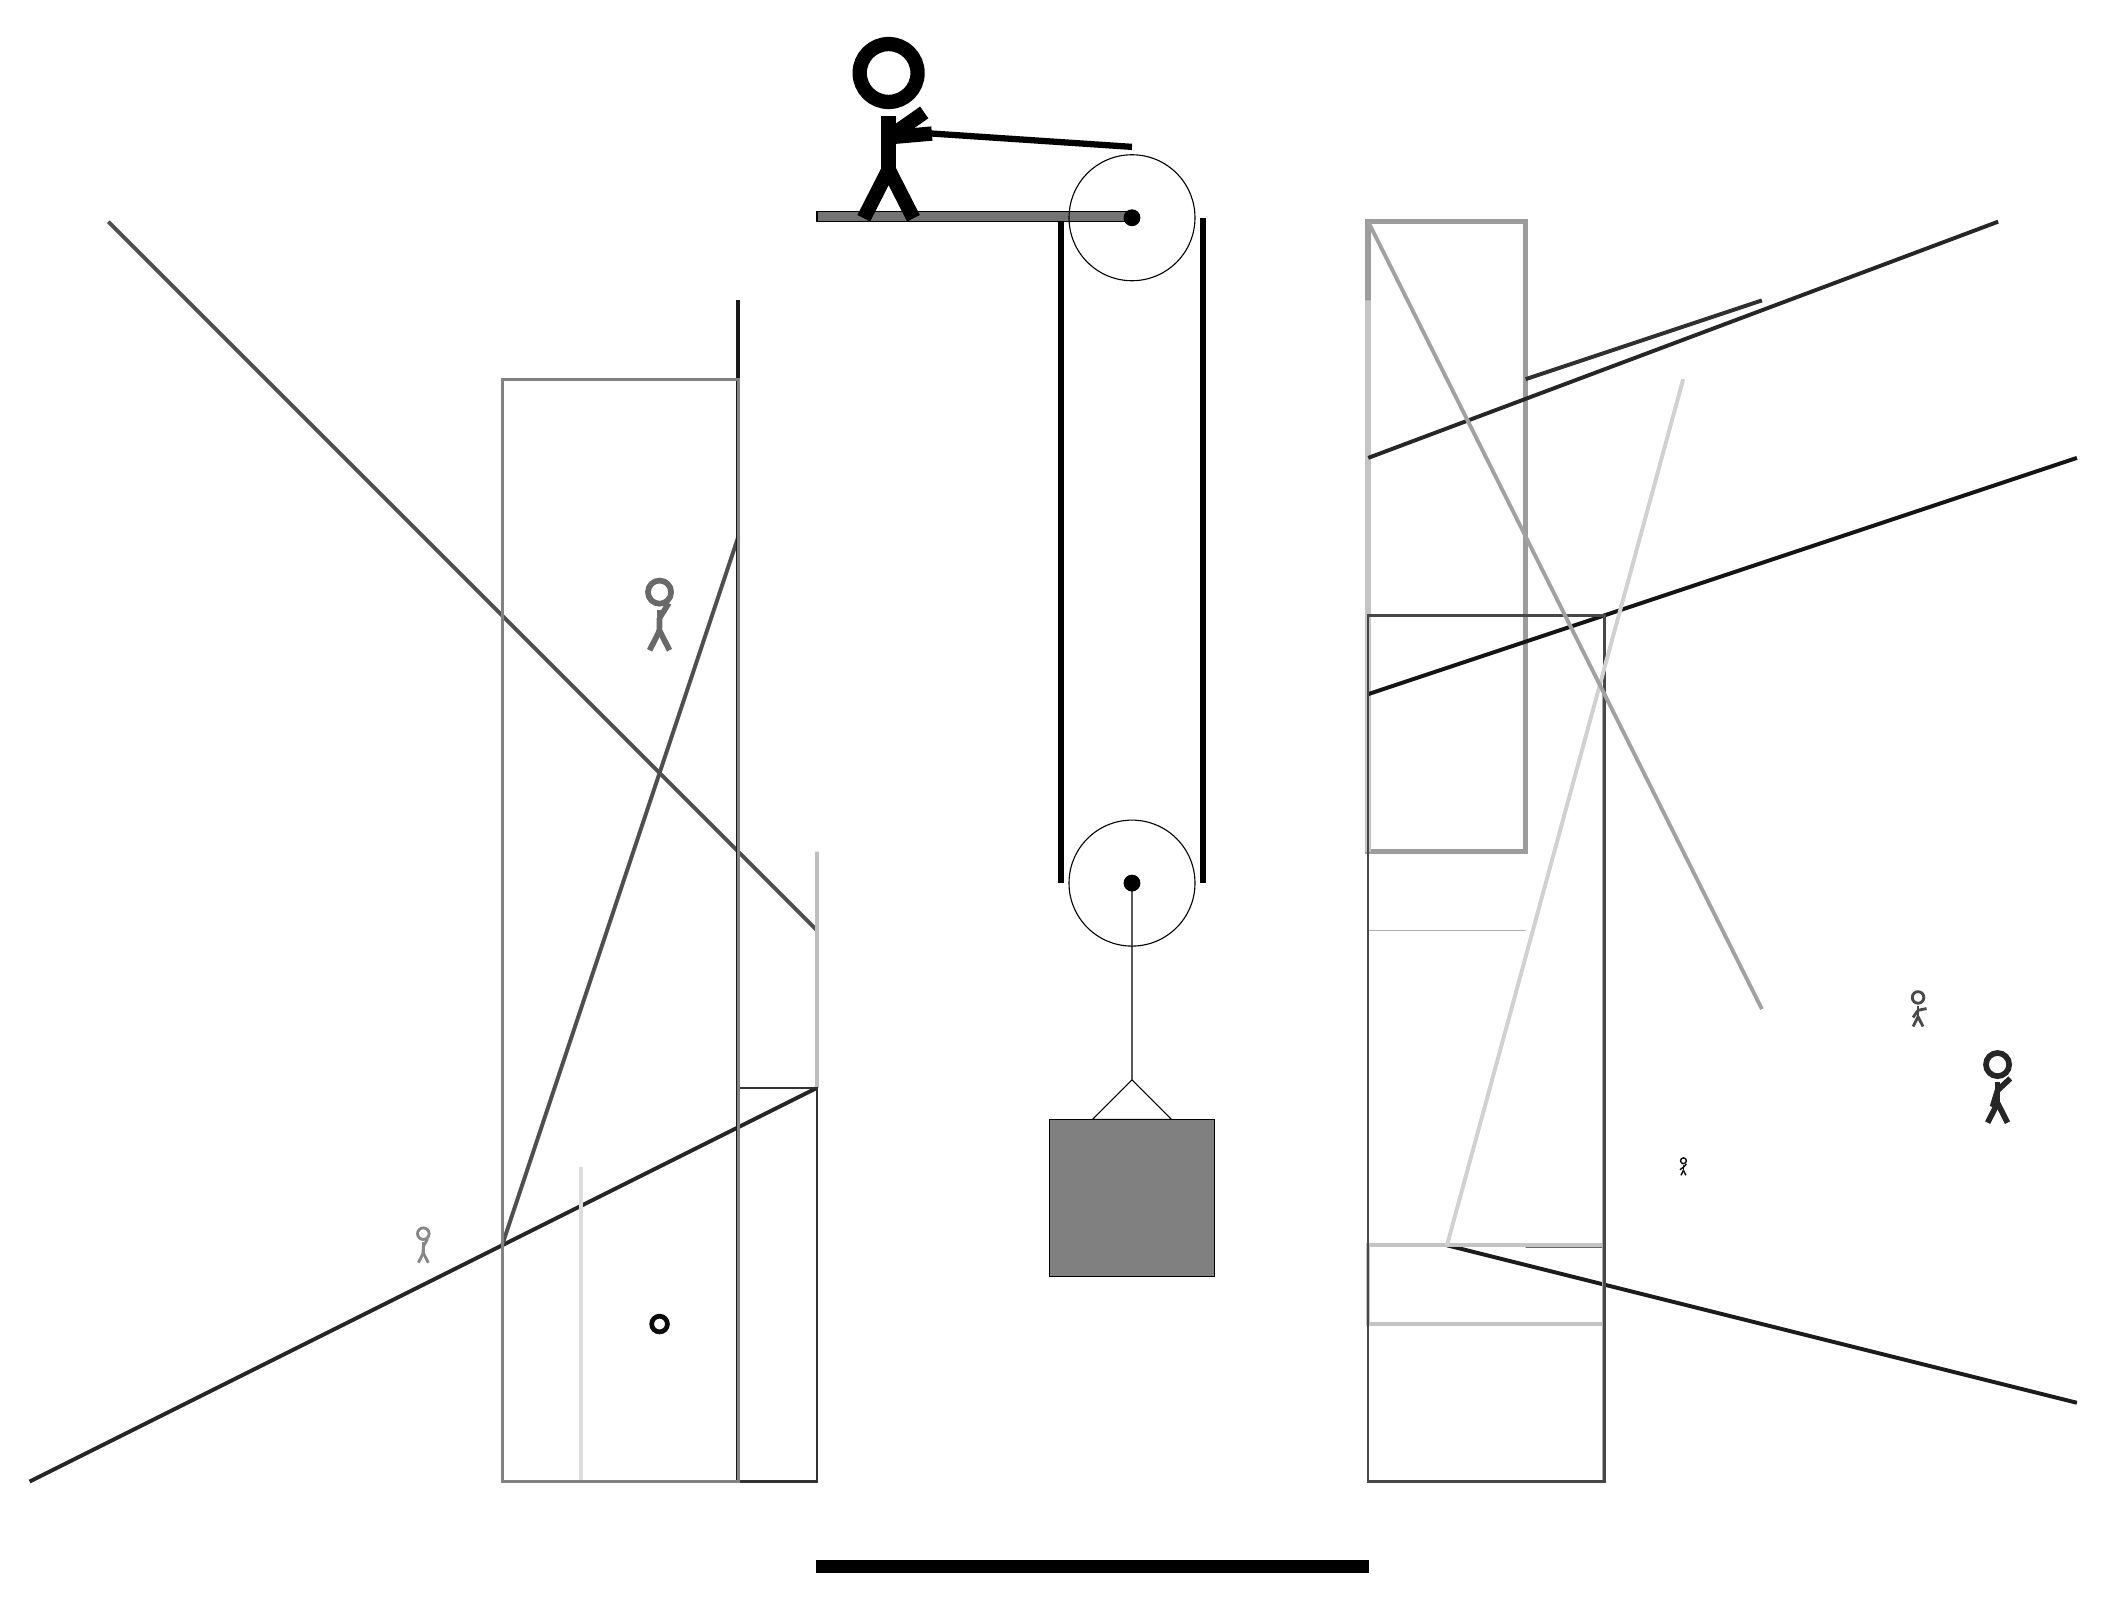
\begin{tikzpicture}
			%%%%% START %%%%%
			
			\draw[fill=black!55] (-2, 14) rectangle (2, 14.125);
			
			\draw (2, 5.6) circle (0.8);
			\draw[fill=black] (2, 5.6) circle (0.1);
			
			\draw (2, 14.05) circle (0.8);
			\draw[fill=black] (2, 14.05) circle (0.1);
			
			\draw (2, 5.6) -- (2, 3.1) -- (1.5, 2.6) -- (2.5, 2.6) -- (2, 3.1);
			\draw[fill=black!50] (0.95, 2.6) rectangle (3.05, 0.6);
			
			\draw[line width=0.8mm] (1.1, 14) -- (1.1, 5.6);
			\centerarc[line width=0.8mm](2, 5.6)(180:360:0.9);
			\draw[line width=0.8mm](2.9, 5.6) -- (2.9, 14.05);
			\centerarc[line width=0.8mm](2, 14.05)(0:90:0.9);
			\draw[line width=0.8mm](2, 14.95) -- (-1, 15.15);
			
			\node at (-1, 15.15) {\Strichmaxerl[10][-175][35]};
			
			\draw[line width=0.5mm, color=black!85](-2, 3) -- (-12, -2);
			
			\draw[line width=0.5mm, color=black!69](-2, 5) -- (-11, 14);
			\draw[line width=0.5mm, color=black!89](6, 1) -- (14, -1);
			\draw[line width=0.6mm, color=black!59] (7, 1) rectangle (8, 1);
			
			\draw[line width=0.7mm, color=black!39] (7, 14) rectangle (5, 6);
			\draw[line width=0.6mm, color=black!25] (-2, 3) rectangle (-2, 6);
			\node[line width=0.5mm, color=black!47] at (-7, 1) {\Strichmaxerl[2][87][61]};
			\draw[line width=0.3mm, color=black!80] (-2, -2) rectangle (-3, 3);
			\draw[line width=0.7mm, color=black!23] (5, 6) rectangle (5, 13);
			
			\draw[line width=0.5mm, color=black!23] (5, 1) rectangle (8, 0);
			\node[line width=0.4mm, color=black!85] at (13, 3) {\Strichmaxerl[4][73][43]};
			
			\draw[line width=0.2mm, color=black!31] (5, 5) rectangle (7, 5);
			\draw[line width=0.5mm, color=black!85](5, 11) -- (13, 14);
			
			\node[line width=0.5mm, color=black!59] at (-4, 9) {\Strichmaxerl[4][89][58]};
			\draw[line width=0.5mm, color=black!33](8, -2) -- (8, 8);
			\draw[line width=0.5mm, color=black!81](10, 13) -- (7, 12);
			
			\draw[line width=0.5mm, color=black!69](-3, 10) -- (-6, 1);
			
			\draw[line width=0.5mm, color=black!90](-3, -2) -- (-3, 13);
			\draw[line width=0.5mm, color=black!92](5, 8) -- (14, 11);
			\draw[line width=0.3mm, color=black!72] (5, -2) rectangle (8, 9);
			\draw[line width=0.5mm, color=black!18](9, 12) -- (6, 1);
			
			\draw[line width=0.5mm, color=black!13](-5, -2) -- (-5, 2);
			\node[line width=0.7mm, color=black!71] at (12, 4) {\Strichmaxerl[2][55][12]};
			\draw[line width=0.5mm, color=black!37](5, 14) -- (10, 4);
			\draw [line width=0.6mm, color=black!96](-4, 0) circle (0.1);
			
			\draw [line width=0.3mm, color=black!88](6, 2) circle (0.0);
			
			\node[line width=0.2mm, color=black!94] at (9, 2) {\Strichmaxerl[1][36][47]};
			\draw[line width=0.4mm, color=black!49] (-3, 12) rectangle (-6, -2);
			
			
			\draw[fill=black] (-2, -3) rectangle (5, -3.15);
			
			%%%%% END %%%%%
		\end{tikzpicture}
	\end{figure}	
\end{document}